%% ----------------------------------------------------------------
%% PACKAGES
%% ----------------------------------------------------------------
\documentclass[titlepage, 12pt]{article}
\usepackage[dvipsnames]{xcolor}     %first needed because tikz
\usepackage[utf8]{inputenc}
\usepackage[spanish]{babel}
\usepackage{amsmath}
\usepackage{biblatex}
\usepackage{booktabs}
\usepackage[RPvoltages]{circuitikz}
\usepackage{csquotes}   %used by biblatex
\usepackage{enumitem}
\usepackage{fancyhdr}
\usepackage{float}
\usepackage{geometry}
\usepackage{graphicx}
\usepackage[hidelinks]{hyperref}
\usepackage{parskip}
\usepackage{siunitx}
\usepackage{subcaption}
\usepackage{subfiles}
\usepackage{tikz}
\usepackage{xfrac}
\usepackage[dvipsnames]{xcolor}

% Custom package for non italic uppercase
% inside equations
%%\usepackage{nonitalic_upper}

%% ----------------------------------------------------------------
%% PACKAGE SETTINGS
%% ----------------------------------------------------------------
\decimalpoint
\geometry{
 a4paper,
 total={170mm,247mm},   %210x297mm
 left=20mm,
 top=20mm,
}
%\setlength\headheight{30pt}
\addbibresource{bibliography.bib}


%% ----------------------------------------------------------------
%% TITLE
%% ----------------------------------------------------------------
\title{Calibrador y caracterizador de sondas de corriente}
\author{Agustín Aon Sanchez\\
Facultad de Ingeniería\\
Universidad Nacional de Mar del Plata}
\date{Director: Dr. Ignacio Carugati}

%% ----------------------------------------------------------------
%% BEGIN
%% ----------------------------------------------------------------
\begin{document}
\maketitle

% Add more spacing
\renewcommand{\baselinestretch}{1.25}\normalsize
\tableofcontents
\renewcommand{\baselinestretch}{1.0}\normalsize

\newpage

\usetikzlibrary{shapes, arrows, babel}
\tikzstyle{block} = [draw, fill=gray!5, rectangle, minimum height=3em, minimum width=6em]
\tikzstyle{sum} = [draw, fill=gray!10, circle, node distance=2cm]
\tikzstyle{input} = [coordinate]
\tikzstyle{output} = [coordinate]
\tikzstyle{pinstyle} = [pin edge={to-,thin,black}]
\tikzstyle{branch} = [circle,inner sep=0pt,minimum size=1mm,fill=black,draw=black]

\def\normalcoord(#1){coordinate(#1)}
\def\showcoord(#1){node[circle, red, draw, inner sep=1pt, pin={[red, overlay, inner sep=0.5pt, font=\tiny, pin distance=0.1cm, pin edge={red, overlay}]45:#1}](#1){}}
\let\coord=\normalcoord

\renewcommand{\listtablename}{Índice de tablas}
\renewcommand{\tablename}{Tabla}
%\setcounter{secnumdepth}{5}        % paragraph con numeros

%% ----------------------------------------------------------------
%% DOCUMENT
%% ----------------------------------------------------------------

%% ----------------------------------------------------------------
\section{Resumen}
%% ----------------------------------------------------------------
En este trabajo se presenta el diseño e implementación de un banco para la calibración y caracterización de sondas de corriente. El hardware contiene un microcontrolador ARM SAM4S, puerto mini USB, un conversor analógico-digital y un generador de corriente utilizando una configuración tipo puente-H. Se describe además el desarrollo del firmware del microcontrolador y el software en PC.

%% ----------------------------------------------------------------
\section{Introducción}
%% ----------------------------------------------------------------
\subfile{sections/introduccion}


%% ----------------------------------------------------------------
\section{Anteproyecto}
%% ----------------------------------------------------------------

  %% ----------------------------------------------------------------
  \subsection{Objetivo general}
  %% ----------------------------------------------------------------
  Diseño y construcción de un banco de calibración y caracterización de sondas de corriente utilizadas en equipos de calidad de energía. El diseño contempla el desarrollo de hardware dedicado, firmware y una aplicación de usuario (software).

  %% ----------------------------------------------------------------
  \subsection{Objetivos específicos}
  %% ----------------------------------------------------------------

      \begin{itemize}
          \item Realizar un estudio del instrumento a construir.
          \item Crear un diagrama en bloques del funcionamiento del equipo.
          \item Diseñar el hardware necesario en base al equipamiento disponible. Se debe diseñar el circuito y PCB que logren una precisión acorde a los requerimientos.
          \item Programar el firmware del microcontrolador. Se desarrollará el código que comandará las tareas de medición en el banco. Entre ellas: lazo de control, procesamiento digital de señales, manejo de gran cantidad de datos y técnicas de comunicaciones.
          \item Programar la interfaz gráfica para controlar el equipo a diseñar desde la PC. Se seleccionarán los tipos de ensayo a realizar (respuesta en frecuencia, respuesta al escalón, distorsión armónica, entre otros) y se mostrarán los resultados generando un informe en formato a definir.
          \item Armado del banco. Se realizará considerando aspectos mecánicos, seguridad eléctrica y demás criterios necesarios.
          \item Realizar la calibración del equipo.
      \end{itemize}

  %% ----------------------------------------------------------------
  \subsection{Características de diseño}
  %% ----------------------------------------------------------------
  El banco debe proveer de las herramientas necesarias para calibrar y caracterizar sondas de corriente. Estas se conectarán al banco y el mismo debe realizar las tareas definidas por el usuario y proveer de la información solicitada eliminandó tareas manuales.

  Los principales requerimientos para las corrientes generadas por el instrumento son:

      \begin{itemize}
          \item Error de 0.1\% de amplitud y fase
          \item Rango de frecuencias de \SI{50}{Hz} a \SI{2000}{Hz}
          \item Corriente de set point de \SI{1}{Arms} a \SI{400}{Arms}
      \end{itemize}

  A fines de cumplir con estas características, se planteó un diagrama en bloques del sistema, el cual se puede ver en la \autoref{fig:bloques-general}.

      \begin{figure}[!htbp]
          \centering
          \includegraphics[width=\textwidth]{diagrams/bloques-general.png}
          \caption{Diagrama en bloques general del sistema}
          \label{fig:bloques-general}
      \end{figure}

  El instrumento contará con un microcontrolador que realizará el control digital de todas las operaciones, proveerá de una interfaz USB para el control del dispositivo a través de una PC y generará los perfiles de corriente para los diferentes ensayos.

  El puente H generará la corriente necesaria, realizando un switcheo de tensión de alta frecuencia. Será controlado por los puertos PWM del microcontrolador, que permitirán realizar un ajuste fino de parámetros tales como el dead time.

  La salida de corriente del puente H pasará por un multiplicador similar al visto en la \autoref{fig:fluke-5500a-foto}, en donde su magnitud pueda aumentarse significativamente y así llevar a fondo de escala a las bobinas de Rogowski. Además, de manera de poder realizar un control, se colocará una resistencia shunt en serie que permita medir esta corriente para cerrar el lazo.

  Los circuitos de adecuación y filtrado proveerán del offset y ganancias necesarios para poder realizar las mediciones correctamente, además de realizar un filtrado antialising. Se deberá contar con 4 canales, de manera de tener uno para el sensor de corriente tipo resistencia shunt, uno para la sonda de corriente y dos canales adicionales para otros instrumentos que se quieran calibrar o caracterizar.

  La salida de estos circuitos de adecuación y filtrado será muestreada por un conversor analógico digital de 16 bits, que proveerá la señal digitalizada al microcontrolador, para su posterior procesado y envío de resultados a la PC.

  En la siguiente sección se procede a explicar el funcionamiento y elección de cada uno de estos bloques principales incluídos en el banco de calibración.

%% ----------------------------------------------------------------
\section{Proyecto}
%% ----------------------------------------------------------------
En este capítulo se describe el diseño del calibrador y caracterizador de sondas de corriente. Para una mejor lectura se ha dividido el mismo en las siguientes tres secciones:

    \begin{itemize}
        \item Diseño analógico y digital
        \item Diseño de firmware
        \item Diseño de software
    \end{itemize}

A continuación se describirá el proceso de diseño llevado a cabo.


  %% ----------------------------------------------------------------
  \subsection{Diseño analógico y digital}
  %% ----------------------------------------------------------------

    %% ----------------------------------------------------------------
    \subsubsection{Fuentes de alimentación}
    %% ----------------------------------------------------------------
    Observando las necesidades de alimentación de los componentes elegidos, se tomó nota de las tensiones a generar para poder proveerlas:
        \begin{itemize}
            \item Fuente de alimentación de \SI{24}{V} (externa)
            \item Fuente de alimentación de \SI{12}{V}
            \item Fuente de alimentación de \SI{5}{V}
            \item Fuente de alimentación de \SI{-5}{V}
            \item Fuente de alimentación de \SI{3.3}{V}
            \item Fuente de alimentación de \SI{1.8}{V}
        \end{itemize}

      %% ----------------------------------------------------------------
      %% PÁRRAFO
      %% ----------------------------------------------------------------
      \paragraph{Fuente de alimentación de 24V (externa)}
      %% ----------------------------------------------------------------
      Esta fuente se encargará de alimentar todo el circuito. Dado que este es un instrumento de banco, no se necesitaba que tuviera una conexión a la red propia, de manera que para ahorrar componentes se decidió este camino.

      De acuerdo a simulaciones realizadas, la fuente de alimentación externa debe proveer al menos \SI{2}{A}, con un margen de seguridad, de manera de poder comopensar las pérdidas ocurridas en la conmutación.

%% ----------------------------------------------------------------
%% PÁRRAFO
%% ----------------------------------------------------------------
\paragraph{Fuente de alimentación de 12V}
%% ----------------------------------------------------------------
Esta fuente se encarga de alimentar la fuente de \SI{5}{V} y el driver del MOSFET. Se eligió una fuente de tipo switching, ya que se alimenta directamente desde la entrada de \SI{12}{V} y alimenta indirectamente todo el PCB.

Se eligió el integrado LM22673TJ-ADJ. El mismo tiene las siguientes características:
  \begin{itemize}
    \item Amplia tensión de entrada: \SI{4.5}{V} - \SI{42}{V}
    \item Tensión de salida ajustable a partir de resistencias de feedback
    \item Precisión de $\pm 1.5 \%$
    \item Corriente continua máxima de \SI{3}{A}
    \item Corriente pico ajustable
  \end{itemize}

En la \autoref{fig:analog-lm22673-bloques} se puede observar el diagrama de bloques funcional del integrado LM22673-TJ-ADJ, brindado por el fabricante en la hoja de datos.

  \begin{figure}[!htbp]
    \centering
    \includegraphics[scale=0.5]{images/analog-lm22673-bloques}
    \caption{Diagrama de bloques del integrado LM22673-TJ-ADJ}
    \label{fig:analog-lm22673-bloques}
  \end{figure}

En la \autoref{fig:analog-fuente-12v} se puede observar el esquemático de la fuente de \SI{12}{V}.

  \begin{figure}[!htbp]
    \centering
    \includegraphics[scale=0.55]{images/analog-fuente-12v}
    \caption{Fuente de alimentación de \SI{12}{V}}
    \label{fig:analog-fuente-12v}
  \end{figure}

Siguiendo las indicaciones de la hoja de datos, se procedió a elegir los componentes:

  \begin{itemize}

    \item $C_2$ y $C_3$ conectados a $V_{IN}$. Esta combinación de capacitores de desacoplamiento, uno electrolítico grande y uno cerámico más pequeño, permite aislar al circuito de ruidos tanto de baja como de alta frecuencia provenientes de la fuente de tensión. También permite compensar las inductancias parásitas.

    \item $R_2$ conectado a $I_{ADJ}$. Este pin regula la corriente máxima pico. Una solo resistencia es necesaria entre este pin y masa para poder controlarla, de acuerdo a lo mostrado en la \autoref{fig:analog-lm22673-iadj}.

      \begin{figure}[!htbp]
        \centering
        \includegraphics[scale=0.6]{images/analog-lm22673-iadj.png}
        \caption{Corriente pico máxima vs. resistencia de $I_{ADJ}$ en LM22673-TJ-ADJ}
        \label{fig:analog-lm22673-iadj}
      \end{figure}

    \item $R_1$ y $R_3$ conectados a $FB$. Este pin permite ajustar la tensión generada, a partir de la correcta elección de valores de las resistencias. Se siguió la siguiente ecuación provista por el fabricante, siendo $R_{FBT}$ la resistencia entre $FB$ y $V_{OUT}$ y $R_{FBB}$ la resistencia entre $FB$ y masa.
      \[
        R_{FBT} = \left[ \frac{V_{out}}{1.285} - 1 \right] \cdot R_{FBB}
      \]

    \item $L_1$, $C_5$, $C_6$ y $C_7$ conectados a $SW$ formando así un filtro pasabajos para generar la tensión de salida.

    \item $C_1$ y $D_1$ conectados entre $BOOT$ y $SW$ y entre $SW$ y masa respectivamente. Este capacitor de bootstrapping genera en conjunto con el diodo la tensión necesaria para encender el MOSFET que se encuentra a la salida del integrado, tal como se observa en la \autoref{fig:analog-lm22673-bloques}. Se eligió además un diodo tipo Schottky, de acuerdo a las recomendaciones del fabricante, con una tensión reversa máxima  de 1.3 veces la máxima tensión de entrada.

    \item $C_4$ conectado a $SS$. Este pin permite regular la función \emph{soft-start} del integrado, reduciendo el tiempo que le toma llegar a estado estacionario y de esa forma someter a menor estrés al mismo. Fue elegido siguiendo la siguiente ecuación:
      \[
        T_{SS} \approx \num{26e3} \cdot C_{SS}
      \]
    tomando el máximo valor recomendado por el fabricante (de \SI{100}{nF} a \SI{1}{\micro F}), ya que no se necesitan mejores prestaciones.

    \end{itemize}

      %% ----------------------------------------------------------------
      %% PÁRRAFO
      %% ----------------------------------------------------------------
      \paragraph{Fuente de alimentación de 5V y 1.8V}
      %% ----------------------------------------------------------------
      La fuente de \SI{5}{V} alimenta el conversor analógico digital, las fuentes de \SI{3.3}{V}, \SI{1.8}{V}, \SI{-5}{V} y los amplificadores operacionales empleados en la etapa de adquisición y adecuación de señales.

      La fuente de \SI{1.8}{V}, por otro lado, alimenta solamente el ADC.

      Dado el bajo costo y las relativamente bajas necesidades de potencia, se decidio utilizar una fuente lineal. Por motivos de disponibilidad se eligió el integrado LM1117 de tensión fija. El mismo tiene las siguientes características:

          \begin{itemize}
              \item Corriente máxima de \SI{800}{mA}
              \item Máxima regulación de carga del 0.4\%
              \item Mínima cantidad de componentes
          \end{itemize}

      El diagrama de bloques del integrado se puede ver en la \autoref{fig:analog-lm1117-bloques}

          \begin{figure}[!htbp]
              \centering
              \includegraphics[scale=0.6]{images/analog-lm1117-bloques.png}
              \caption{Diagrama de bloques del integrado LM1117MP-1.8/NOPB}
              \label{fig:analog-lm1117-bloques}
          \end{figure}

      En la \autoref{fig:analog-fuente-1v8} se puede observar el esquemático de la fuente de \SI{1.8}{V}. La versión utilizada del integrado es la LM1117MP-1.8.

          \begin{figure}[!htbp]
              \centering
              \includegraphics[scale=0.6]{images/analog-fuente-1v8.png}
              \caption{Fuente de alimentación de \SI{1.8}{V}}
              \label{fig:analog-fuente-1v8}
          \end{figure}

      El esquemático de la fuente de \SI{5}{V} es idéntico, siendo en este caso el integrado LM1117MP-5.0, versión de tensión fija para \SI{5}{V}.

      %% ----------------------------------------------------------------
      %% PÁRRAFO
      %% ----------------------------------------------------------------
      \paragraph{Fuente de alimentación de 3.3V}
      %% ----------------------------------------------------------------
      Esta fuente alimenta las siguientes partes del circuito: microcontrolador, ADC y driver del MOSFET. Dados los bajos requerimientos de potencia y el menor costo, se decidió utilizar una fuente lineal.

      De esta forma se eligió el integrado TPS79533DCQR. El mismo ha sido utilizado en diseños previos con un alto grado de confiabilidad. Entre sus características más destacables se encuentra:

          \begin{itemize}
              \item Corriente máxima de \SI{500}{mA}
              \item Muy bajo ruido (\SI{33}{\micro V_{RMS}})
              \item Baja caída de tensión a máxima carga (\SI{110}{mV})
              \item Mínima cantidad de componentes
          \end{itemize}

      El diagrama en bloques del integrado se puede ver en la \autoref{fig:analog-TPS79533DCQR-bloques}.

          \begin{figure}[!htbp]
              \centering
              \includegraphics[scale=0.5]{images/analog-TPS79533DCQR-bloques.png}
              \caption{Diagrama de bloques del integrado TPS79533DCQR}
              \label{fig:analog-TPS79533DCQR-bloques}
          \end{figure}

      En la \autoref{fig:analog-fuente-3v3} se puede observar el esquemático de la fuente de \SI{3.3}{V}.

          \begin{figure}[!htbp]
              \centering
              \includegraphics[scale=0.5]{images/analog-fuente-3v3.png}
              \caption{Fuente de alimentación de \SI{3.3}{V}}
              \label{fig:analog-fuente-3v3}
          \end{figure}

      Siguiendo las indicaciones de la hoja de datos, se eligieron los componentes necesarios. Estos, tal como se puede observar, son simplemente tres capacitores, ya que este integrado permite un uso mínimo de componentes.

%% ----------------------------------------------------------------
%% SUB-SUB-SECCIÓN
%% ----------------------------------------------------------------
\subsubsection{Etapa de adecuación y filtrado}
\label{sec:adecuacion}
%% ----------------------------------------------------------------
Este circuito provee la ganancia y filtrado anti-aliasing para los cuatro canales del conversor analógico digital. Los mismos, están divididas en dos tipos diferentes:
    \begin{itemize}
        \item Un canal para medir la corriente en el multiplicador. Se mide la caída de tensión de la resistencia shunt colocada en serie con la corriente que circula por la carga. Esta medición es realizada de manera de, a partir de un lazo de control, regular la corriente.
        \item Tres canales para la conexión de las sondas de corriente a caracterizar.
    \end{itemize}

Si bien existen estos dos tipos de entradas, el circuito de adecuación y filtrado es el mismo para todas, pudiendo variar entre ellos la ganancia aplicada.

En la \autoref{fig:adecuacion-circuito} se puede observar el circuito genérico utilizado para la adecuacion y filtrado.

\begin{figure}[!htbp]
    \centering
    \begin{circuitikz}[scale=0.6]
        \ctikzset{resistors/scale=0.6, capacitors/scale=0.6}
        % Primera etapa
        \draw (0,0)     node[op amp]    (U1) {$U_1$};
        \draw (U1.out)  to [short] ++(0.2,0) \coord(U1out);
        \draw (U1.+)    to [short, -*] ++(-1,0) \coord(U1+);
        \draw (U1+)     to [C, l=$C_2$] ++(0,-3) to [short, -o] ++(-4,0) node[left](Vref){$\frac{V_{REF}}{2}$};
        \draw (U1+)     to [short, -*] ++(-2,0) \coord(R2_b) to [R, l=$R_2$] ++(0,-3);
        \draw (R2_b)    to [R, l=$R_1$, -o] ++(-4,0) node[left](V+){$V_{in}^+$};
        \draw (U1.-)    to [short, -*] ++(-1,0) \coord(U1-);
        \draw (U1-)     to [short] ++(-2,0) to [R, l_=$R_1$, -o] ++(-4,0) node[left](V-){$V_{in}^-$};
        \draw (U1-)     to [short, -*] ++(0,2) \coord(tanque1_in);
        \draw (tanque1_in) to [C, l=$C_2$, -*] ++(5,0);
        \draw (tanque1_in) to [short] ++(0,2) to [R, l=$R_2$] ++(5,0) \coord(tanque1_out) to [short, -*] (tanque1_out |- U1out);

        % Segunda etapa
        \draw (U1out)  to [R, -*, l=$R_3$] ++(3,0) \coord(R3_out) to [R, *-, l=$R_3$] ++(0,-3) node[ground](GND){};
        \draw (R3_out) to [R, l=$R_4$, -*] ++(3,0) \coord(R4_out) to [C, l=$C_4$] ++(0,-3) node[ground](GND){};
        \draw (R4_out) to [short] ++(2,0) \coord(U2+) to [short] ++(1,0) \coord(U2);
        \draw (U2) node[op amp, anchor=+, yscale=-1] (U2) {\ctikzflipy{$U_2$}};
        \draw (U2.out) to [short, -*] ++(1,0) \coord(U2out);
        \draw (U2.-) to [short] ++(-1,0) \coord(U2-);
        \draw (U2-) to [short, -*] ++(0,-2) \coord(R5) to [R, l=$R_5$] ++(0,-3) node[ground](GND){};
        \draw (R5) to [R, l=$R_6$] ++(5,0) \coord(R5out) to [short] (R5out |- U2out);
        \draw (R3_out) to [short] ++(0,2) to [C, l=$C_4$] ++(10,0) \coord(C4out) to [short, -*] (C4out |- U2out);
        \draw (U2out) to [short, -o] ++(0,0) node[right](Vout){$V_{out}$};
    \end{circuitikz}
    \caption{Circuito de adecuación y filtrado}
    \label{fig:adecuacion-circuito}
\end{figure}

%% ------------------------
\paragraph{Primera etapa}
%% ------------------------
En esta etapa que culmina en la salida del primer amplificador operacional $U_1$, se incluye una configuración diferencial junto con un filtro pasabajos de primer orden. La transferencia de esta etapa es la siguiente:
\[
    \frac{V_1(s)}{V_{in}^+(s) - V_{in}^-(s)} = \frac{R_2}{R_{1} } \cdot \frac{1}{1+sC_{2}R_{2}}
\]

%% TODO: justificar 3400 Hz
De manera de tener una frecuencia de corte de aproximadamente \SI{3400}{Hz}, se eligieron los siguientes valores:
    \begin{itemize}
        \item $R_2 = \SI{4.7}{k \ohm}$
        \item $C_2 = \SI{10}{nF}$
    \end{itemize}

Se obtuvo de esta forma una frecuencia de corte $f_c = \SI{3386}{Hz}$. La resistencia $R_1$ se elegirá de acuerdo a las necesidades de ganancia de cada entrada.

Los amplificadores operacionales son alimentados en forma unipolar, por lo que se emplea una tensión de offset de $\frac{V_{REF}}{2}$.

\paragraph{Segunda etapa}
Filtro pasabajos de segundo orden tipo Sallen-Key.

Si se observa la \autoref{fig:adecuacion-circuito-sallenkey}, se verá una de las configuraciones más comunes encontradas en la literatura \cite{ti:sloa024b}.

\begin{figure}[!htbp]
    \centering
    \begin{circuitikz}[scale=0.6]
        \ctikzset{resistors/scale=0.6, capacitors/scale=0.6}
        % Segunda etapa
        \draw (0,0) node[left](Vin){$V_i$} to [R, l=$R_3$, o-] ++(4,0) \coord(R3_out);
        \draw (R3_out) to [R, l=$R_4$, *-] ++(3,0) \coord(R4_out) to [C, l=$C_3$, *-] ++(0,-3) node[ground](GND){};
        \draw (R4_out) to [short] ++(2,0) \coord(U2+) to [short] ++(1,0) \coord(U2);
        \draw (U2) node[op amp, anchor=+, yscale=-1] (U2) {\ctikzflipy{$U_2$}};
        \draw (U2.out) to [short] ++(1,0) \coord(U2out);
        \draw (U2.-) to [short] ++(-1,0) \coord(U2-);
        \draw (U2-) to [short, -*] ++(0,-2) \coord(R5) to [R, l=$R_5$] ++(0,-3) node[ground](GND){};
        \draw (R5) to [R, l=$R_6$] ++(5,0) \coord(R5out) to [short, -*] (R5out |- U2out);
        \draw (R3_out) to [short] ++(0,2) to [C, l=$C_4$] ++(10,0) \coord(C4out) to [short] (C4out |- U2out);
        \draw (U2out) to [short, -o] ++(0,0) node[right](Vout){$V_{o}$};
    \end{circuitikz}
    \caption{Configuración Sallen-Key pasabajos estándar}
    \label{fig:adecuacion-circuito-sallenkey}
\end{figure}

La transferencia de un circuito Sallen-Key en la configuración de la \autoref{fig:adecuacion-circuito-sallenkey} es la siguiente:
    \[
        \frac{V_o(s)}{V_i(s)} = \frac{K}{s^2(R_3R_4C_3C_4) + s(R_3C_3+R_4C_3+R_3C_4(1-K)) + 1}
    \]
siendo:
    \[
      f_c = \frac{1}{2\pi \sqrt{R_3R_4C_3C_4}} \qquad \text{y} \qquad Q = \frac{\sqrt{R_3R_4C_3C_4}}{R_3C_3+R_4C_3+R_3C_4(1-K)}
    \]

Para acelerar el diseño, se pueden encontrar en la literatura diversas simplificaciones \cite{ti:sloa024b}. En este caso, se ha decidido optar por igualar componentes. Así, $R_3 = R_4 = R$ y $C_3 = C_4 = C$, resultando en:
    \[
        f_c = \frac{1}{2\pi RC} \qquad \text{y} \qquad Q = \frac{1}{3 - K}
    \]

Así, se eligió utilizar un factor $Q=1$ que, utilizando resistencias con margen de error de $1 \%$, resultaría para un peor caso un factor $Q=1.02$.

Habiendo realizado esta elección, y siendo este el único grado de libertad del circuito, se obtiene $K=2$. Es por ello que, tal como se mencionó antes, se realiza la modificación en la resistencia $R_3$. Al atenuar la señal a la mitad con el divisor resistivo antes de introducirla a la segunda etapa, se cancela el efecto de ganancia de esta última, quedando así, a fines prácticos, una ganancia unitaria. La única condición necesaria es ahora:
    \[
        \frac{R_3}{2} = R_4
    \]
de manera de cumplir la simplificación planteada.

Atendiendo a todas estas consideraciones y cumpliendo la frecuencia de corte antes planteada, se eligieron los siguientes valores:
    \begin{itemize}
        \item $R_3 = \SI{9.31}{k\ohm}$
        \item $R_4 = \SI{4.7}{k\ohm}$
        \item $C_3 = C_4 = \SI{10}{nF}$
        \item $R_5 = R_6 = \SI{10}{k\ohm}$
    \end{itemize}
así utilizando los mismos componentes que en la etapa previa, llegando a la frecuencia de corte de \SI{3386}{Hz}, logrando así el filtro pasabajos de tercer orden deseado.

En la \autoref{fig:adecuacion-circuito-i1} se puede observar finalmente el circuito de adecuación y filtrado elegido para la entrada de corriente 1.

    \begin{figure}[!htbp]
        \centering
        \includegraphics[scale=0.32]{images/adecuacion-circuito.png}
        \caption{Circuito de adecuación y filtrado de la entrada de corriente 1}
        \label{fig:adecuacion-circuito-i1}
    \end{figure}

En el circuito final, se agregaron dos diodos schottky a la salida, uno conectado a \SI{3.3}{V} y el otro a masa para la protección de las entradas del conversor analógico digital, limitando la tensión máxima a $\SI{3.3}{V} + V_F$, siendo $V_{F_{max}} = \SI{1}{V}$ para el integrado elegido.

%% ----------------------------------------------------------------
%% SUB-SUB-SECCIÓN
%% ----------------------------------------------------------------
\subsubsection{Microcontrolador}
%% ----------------------------------------------------------------
El microcontrolador elegido es el SAM4S8B con las siguientes características:
    \begin{itemize}
        \item Frecuencia de clock \SI{120}{MHz}
        \item \SI{512}{Kbytes} de memoria Flash
        \item \SI{128}{Kbytes} de de memoria SRAM
        \item Encapsulado 64LQFP
        \item ADC 12-bit de 11 canales
        \item DAC 12-bit de 2 canales
        \item 47 puertos de entrada y salida (PIOs)
        \item 2 UART
        \item PWM, timers, I2C, SPI, y otras funciones
    \end{itemize}

Se utiliza un microcontrolador debido a la necesidad de poder realizar funciones complejas. De esta forma se implementa en el mismo:

    \begin{itemize}
        \item Control digital
        \item Control de generación de corriente a través de PWM
        \item Interfaz con la PC a través de USB
        \item Generación de clock para el ADC externo a través de PWM
        \item Control de ADC externo utilizando SPI
        \item Muestreo utilizando ADC interno (opcional)
        \item Implementación de botones para debugging
        \item Guardado de información de calibración en EEPROM externa
        \item Muestreo, procesamiento y enviado de datos a la PC
    \end{itemize}

Se decidió utilizar la familia Atmel ya que se contaba con disponibilidad y experiencia en su uso. Este modelo en particular fue elegido por su velocidad, confiabilidad y gran capacidad de Flash y SRAM.

A continuación se describirán las diferentes conexiones del microcontrolador y los componentes asociados.

%% --------------------------------
\paragraph{Fuente de alimentación}
%% --------------------------------
Para poder alimentar al microcontrolador, se utilizó la fuente de \SI{3.3}{V}. De esta manera, se procedió a conectar varios capacitores de desacople, tanto de \SI{10}{\micro F} como de \SI{0.1}{\micro F}, de manera de filtrar los diferentes rangos de frecuencia que estos permiten. En la \autoref{fig:arm-supply} se puede observar los componentes utilizados.

    \begin{figure}[!htbp]
        \centering
        \includegraphics[scale=1.5]{images/arm-supply.png}
        \caption{Alimentación del microcontrolador}
        \label{fig:arm-supply}
    \end{figure}

%% --------------------------------
\paragraph{Fuente de alimentación de referencia del ADC interno}
%% --------------------------------
Se agregó una fuente de referencia para el ADC.Se eligió el integrado ISL21010\_3V0, por su facilidad de uso y disponibilidad. En la \autoref{fig:arm-fuente-ref} se puede observar el esquemático utilizado.

    \begin{figure}[!htbp]
        \centering
        \includegraphics[scale=1.5]{images/arm-fuente-ref.png}
        \caption{Fuente de referencia del ADC del microcontrolador}
        \label{fig:arm-fuente-ref}
    \end{figure}

%% --------------------------------
\paragraph{Puertos de entrada y salida}
%% --------------------------------
En estos pines de entrada y salida es donde está concentradas la mayoría de las funciones que se irán explicando por cada grupo. Las conexiones de ambos puertos se pueden ver en la \autoref{fig:arm-gpio-port-a} y en la \autoref{fig:arm-gpio-port-b}.


    \begin{figure}[!htbp]
        \centering
        \includegraphics[scale=1.5]{images/arm-gpio-port-a.png}
        \caption{Pines del puerto A del microcontrolador}
        \label{fig:arm-gpio-port-a}
    \end{figure}

    \begin{figure}[!htbp]
        \centering
        \includegraphics[scale=1.5]{images/arm-gpio-port-b.png}
        \caption{Pines del puerto B del microcontrolador}
        \label{fig:arm-gpio-port-b}
    \end{figure}

Se han conectado también dos cristales que servirán para control del puerto USB ($Y1$) y para la función RTC del microcontrolador ($Y2$).

Cabe destacar algunas señales que se verán en otras etapas, tales como:
    \begin{itemize}
        \item DRV\_PWM\_H, DRV\_PWM\_L: se conectan a la entrada diferencial de control del driver del MOSFET.
        \item SPI\_MISO, SPI\_SPCK: sirven para comunicación entre el ADC y el microcontrolador.
        \item ADC\_CLK: clock del ADC
    \end{itemize}

%% --------------------------------
\paragraph{Conexión JTAG/SWD}
%% --------------------------------
Se agregaron también las conexiones necesarias para colocar un header JTAG/SWD de manera de poder programar el microcontrolador. Como se puede observar en la \autoref{fig:arm-jtag}, se agregaron también resistencias pull-up de \SI{100}{k\ohm} y un capacitor de desacople en la salida de \SI{3.3}{V}.

    \begin{figure}[!htbp]
        \centering
        \includegraphics[scale=1.5]{images/arm-jtag.png}
        \caption{Conexión JTAG/SWD del microcontrolador}
        \label{fig:arm-jtag}
    \end{figure}

%% --------------------------------
\paragraph{Conexión USB}
%% --------------------------------
La conexión USB consta de 2 señales:
    \begin{itemize}
        \item USB\_VBUS: genera la interrupción en el microcontrolador cuando el puerto USB es conectado a la PC, teniendo que adecuarse la tensión de \SI{5}{V} de entrada con un divisor resistivo.
        \item USB\_DD: señal diferencial de transmisión de datos, terminada cada una con una resistencia de \SI{22}{\ohm} de manera de mejorar la adaptación de impedancias.
    \end{itemize}

Se utilizó en este caso un puerto mini-USB, siendo uno de los más usados y comunes en la industria. En la \autoref{fig:arm-usb} se puede observar el esquemático.

    \begin{figure}[!htbp]
        \centering
        \includegraphics[scale=1.5]{images/arm-usb.png}
        \caption{Conexión USB del microcontrolador}
        \label{fig:arm-usb}
    \end{figure}

%% --------------------------------
\paragraph{EEPROM}
%% --------------------------------
Se ha optado por utilizar una memoria EEPROM para guardar los datos de calibración del instrumento. Se conecta mediante I$^2$C.

En la \autoref{fig:arm-eeprom} se puede observar los componentes utilizados. Se agregaron dos resistencias pull-up y un capacitor de desacople.

    \begin{figure}[!htbp]
        \centering
        \includegraphics[scale=1.5]{images/arm-eeprom.png}
        \caption{Conexión EEPROM al microcontrolador}
        \label{fig:arm-eeprom}
    \end{figure}

 %% --------------------------------
 \paragraph{RESET y ERASE}
 %% --------------------------------
Se dejaron dos header expuestos, con el objetivo de tener fácil acceso en caso de graves problemas en el microcontrolador. Estas conexiones son las de RESET y ERASE, permitiendo reiniciar y borrar la memoria, respectivamente. En ambos casos no fue necesario agregar una resistencia de pull-up o pull-down, ya que el microcontrolador las trae integradas dentro del mismo.

En la \autoref{fig:arm-reset-erase} se pueden observar ambos header.

    \begin{figure}[!htbp]
        \centering
        \includegraphics[scale=1.5]{images/arm-reset-erase.png}
        \caption{Header RESET y ERASE del microcontrolador}
        \label{fig:arm-reset-erase}
    \end{figure}

 %% --------------------------------
 \paragraph{Otras conexiones}
 %% --------------------------------
 Además de las ya nombradas, se dejaron ciertos pines expuestos para tener mayor flexibilidad ante futuros cambios:
    \begin{itemize}
        \item Header que deja expuesto el DAC, ADC, UART y demás pines generales de entrada y salida, como se puede ver en la \autoref{fig:arm-header}.
        \item Botón, se puede ver en la \autoref{fig:arm-button}.
        \item LEDs, se puede ver en la \autoref{fig:arm-leds}.
    \end{itemize}

    \begin{figure}[!htbp]
        \begin{subfigure}[b]{\textwidth}
            \centering
            \includegraphics[scale=1.1]{images/arm-header.png}
            \caption{Header}
            \label{fig:arm-header}
        \end{subfigure}

        \begin{subfigure}[b]{0.49\textwidth}
            \centering
            \includegraphics[scale=1.1]{images/arm-button.png}
            \caption{Botón}
            \label{fig:arm-button}
        \end{subfigure}
        \begin{subfigure}[b]{0.49\textwidth}
            \centering
            \includegraphics[scale=1.1]{images/arm-leds.png}
            \caption{LEDs}
            \label{fig:arm-leds}
        \end{subfigure}
        \caption{Otras conexiones del microcontrolador}
    \end{figure}

%% ----------------------------------------------------------------
%% SUB-SUB-SECCIÓN
%% ----------------------------------------------------------------
\subsubsection{ADC}
%% ----------------------------------------------------------------
Para la implementación del lazo de control de corriente en el multiplicador y la adquisición de la señal entregada por la sonda de corriente a caracterizar, se utilizará un conversor analógico digital.

Se eligió el integrado ADS1174IPAPT. Este cuenta con las siguientes características:
    \begin{itemize}
        \item 4 canales simultáneos.
        \item Dos modos de selección posibles: \SI{52}{kSPS} o \SI{10}{kSPS}.
        \item DC Performance:
        \begin{itemize}
            \item \SI{2}{\micro V/\degree C} deriva de offset
            \item \SI{2}{ppm/\degree C} deriva de ganancia
        \end{itemize}

        \item AC Performance:
        \begin{itemize}
            \item \SI{25}{kHz} de ancho de banda
            \item \SI{97}{dB} de SNR
            \item \SI{-105}{dB} de THD
        \end{itemize}
        \item Interfaz SPI.
        \item Muestreador tipo delta-sigma.
        \item Filtro interno de \SI{\pm 0.005}{dB} de ripple y respuesta de fase lineal.
    \end{itemize}

En la \autoref{fig:adc-bloques} se puede observar el diagrama en bloques interno del integrado, provisto por el fabricante.

    \begin{figure}[!htbp]
        \centering
        \includegraphics[scale=0.5]{images/adc-bloques.png}
        \caption{Diagrama en bloques interno del ADS1174IPAPT}
        \label{fig:adc-bloques}
    \end{figure}

%% ------------------------
\paragraph{Alimentación}
%% ------------------------
Este dispositivo, necesita tres fuentes de alimentación separadas: \SI{5}{V}, \SI{3.3}{V} y \SI{1.8}{V}. Debido a indicaciones del fabricante, se agregó un capacitor de desacople de \SI{10}{\micro F} entre cada entrada y masa, como se puede ver en la \autoref{fig:adc-supply}

    \begin{figure}[!htbp]
        \centering
        \includegraphics[scale=1.5]{images/adc-supply.png}
        \caption{Alimentación del ADC}
        \label{fig:adc-supply}
    \end{figure}

%% ------------------------
\paragraph{Entradas analógicas}
%% ------------------------
En el caso de las entradas analógicas, se colocó un capacitor cerámico de \SI{2.2}{nF} entre cada entrada diferencial, por indicación del fabricante para mejorar la performance del sistema. Además, se colocaron las cuatro entradas superiores (AINP4-AINP8) a masa, ya que éstas sólo están habilitadas en la versión de 8 canales del integrado. En esta etapa se incluyó también la tensión de referencia, la cual dictará el fondo de escala del dispositivo. El esquemático resultante se puede ver en la \autoref{fig:adc-inputs}.

    \begin{figure}[!htbp]
        \centering
        \includegraphics[scale=1.5]{images/adc-inputs.png}
        \caption{Entradas analógicas del ADC}
        \label{fig:adc-inputs}
    \end{figure}

%% ------------------------
\paragraph{Entradas/salidas digitales}
%% ------------------------
Siguiendo las indicaciones del fabricante, se conectó el pin DOUT1 a la entrada SPI\_MISO (Master Input Slave Output) del microcontrolador, terminando la conexión con una resistencia de \SI{100}{\ohm} para adaptación de impedancias. Se conectó también SPCK al clock del SPI del microcontrolador y CLK al clock generado por el PWM del microcontrolador. El pin de DRDY (data ready) se ha conectado a una entrada GPIO del microcontrolador.

El funcionamiento de la interfaz SPI es el siguiente. Una vez que el ADC tiene los datos listos, genera una interrupción en el microcontrolador a través del pin de DRDY. El microcontrolador así comienza a generar el clock del SPI y el ADC envía los datos. En la \autoref{fig:adc-spi-tdm} se puede observar una descripción gráfica del funcionamiento descripto.

    \begin{figure}[!htbp]
        \centering
        \includegraphics[scale=0.4]{images/adc-spi-tdm.png}
        \caption{Diagrama de tiempo de envío de datos del ADC en modo TDM}
        \label{fig:adc-spi-tdm}
    \end{figure}

%% ------------------------1
\paragraph{Modos de salida de datos}
%% ------------------------
Tanto para la conexión mediante el protocolo SPI o Frame-Sync, el ADC ofrece tres modos distintos para envío de datos:
    \begin{itemize}
        \item TDM Dynamic: solo se enviarán las muestras de los canales habilitados en serie a través del pin DOUT1.
        \item TDM Fixed: las muestras de \emph{todos} los canales son enviadas en serie a través del pin DOUT1. En caso de que alguno no esté habilitado, se dejará lugar para el tiempo que hubiese ocupado.
        \item Discrete:  las muestras son enviadas en paralelo en cada una de los pones de salida disponibles para tal fin (DOUT1-4).
    \end{itemize}

Previendo futuras modificaciones en el modo de envío de información, se decidió dejar un header que permita modificar esta configuración mediante el agregado de jumpers, como se puede ver en la \autoref{fig:adc-mode-selector}

    \begin{figure}[!htbp]
        \centering
        \includegraphics[scale=1.5]{images/adc-mode-selector.png}
        \caption{Selector de modo de salida de datos del ADC}
        \label{fig:adc-mode-selector}
    \end{figure}

%% ------------------------
\paragraph{Modo de testeo}
%% ------------------------
Este modo permite medir la continudad de los pines de entrada y salida según se ve en la \autoref{tab:adc-test-pins}. Una vez activado, las funciones normales de los pines digitales son deshabilitadas. Nuevamente se dejó un header con pines expuestos en caso de que se necesite utilizar esta función, como se puede ver en la \autoref{fig:adc-test-selector}.

    \begin{table}[!htbp]
        \centering
        \begin{tabular}{|c|c|}
        \hline
        \textbf{Entrada}                 & \textbf{Salida}                 \\ \hline
        PWDN1                            & DOUT1                           \\ \hline
        PWDN2                            & DOUT2                           \\ \hline
        PWDN3                            & DOUT3                           \\ \hline
        PWDN4                            & DOUT4                           \\ \hline
        MODE                             & DIN                             \\ \hline
        FORMAT0                          & CLKDIV                          \\ \hline
        FORMAT1                          & DRDY/FSYNC                      \\ \hline
        FORMAT2                          & SCLK                            \\ \hline
        \end{tabular}
        \caption{Conexión interna de pines en modo de testeo del ADC}
        \label{tab:adc-test-pins}
    \end{table}

    \begin{figure}[!htbp]
        \centering
        \includegraphics[scale=1.5]{images/adc-test-selector.png}
        \caption{Selector de modo de testeo del ADC}
        \label{fig:adc-test-selector}
    \end{figure}

%% ------------------------
\paragraph{Selección de ADC}
%% ------------------------
Se contempló el uso del conversor analógico interno del microcontrolador, por lo que se adicionó un header de selección. El esquemático se puede ver en la \autoref{fig:adc-source-selector}.

    \begin{figure}[!htbp]
        \centering
        \includegraphics[scale=1.5]{images/adc-source-selector.png}
        \caption{Selector de ADC}
        \label{fig:adc-source-selector}
    \end{figure}

%% ----------------------------------------------------------------
%% SUB-SUB-SECCIÓN
%% ----------------------------------------------------------------
\subsubsection{Generación de corriente}
%% ----------------------------------------------------------------
La etapa de generación de corriente se implementó utilizando una configuración puente H. El circuito se puede ver en la \autoref{fig:generacion-corriente}.

\begin{figure}[!htbp]
    \centering
    \begin{circuitikz}[scale=0.6]
        \ctikzset{resistors/scale=0.55, capacitors/scale=0.55}
        \ctikzset{multipoles/thickness=3}
        \ctikzset{multipoles/dipchip/width=1.85}
        \ctikzset{transistors/scale=0.65}

        % uC
        \draw (0,0) node[dipchip, num pins=10, hide numbers, no topmark, external pins width=0](uC){$\mu$C};
        \node [right, font=\tiny] at (uC.bpin 3) {FB}; \draw (uC.bpin 3) to [short] ++(-0.5,0) \coord(uC_fb);
        \node [left, font=\tiny] at (uC.bpin 9) {PWM1}; \draw (uC.bpin 9) to [short] ++(0.5,0) \coord(uC_out1);
        \node [left, font=\tiny] at (uC.bpin 7) {PWM2}; \draw (uC.bpin 7) to [short] ++(0.5,0) \coord(uC_out2);

        % mosfet driver 1
        \draw (uC_out1) to [short] ++(1,0) \coord(md_in) to [short] ++(0.5,0) \coord(md);
        \draw (md) node[dipchip, num pins=10, hide numbers, no topmark, external pins width=0, align=center, font=\scriptsize, anchor=bpin 3] (md){MOSFET\\driver 1};
        \node [right, font=\tiny] at (md.bpin 3) {IN};
        \node [left, font=\tiny] at (md.bpin 9) {OUT1}; \draw (md.bpin 9) to [short] ++(0.5,0) \coord(md_out1);
        \node [left, font=\tiny] at (md.bpin 7) {OUT2}; \draw (md.bpin 7) to [short] ++(0.5,0) \coord(md_out2);

        % mosfets 1
        \draw (md_out1) to [short] ++(1,0) node[nigfete, anchor=G](q1){$Q_1$};
        \draw (md_out2) to [short] ++(1,0) node[nigfete, anchor=G](q2){$Q_2$};
        \draw (q1.S) -- (q2.D);
        \draw (q2.S) -- ++(0,-0.5) node[ground](GND){};

        % inductor and shunt
        \draw (q1.S) to [short, *-] ++(1,0) to [L, l=$L$] ++(2,0) -- ++(0.5,0) \coord(shunt_left) to [short] ++(0.5,0)
        to [R, l_=$R_{shunt}$] ++(1,0) to [short] ++(0.5,0) \coord(shunt_right) to [short, -*] ++(1.5,0) \coord(shunt_out);

        % mosfets 2 de arriba
        \draw (shunt_out) node[nigfete, anchor=S, xscale=-1](q3){\scalebox{-1}[1]{$Q_3$}};

        % mosfet driver 2
        \draw (q3.G) to [short] ++(1,0) \coord(md2_in) to [short] ++(0.5,0) \coord(md2);
        \draw (md2) node[dipchip, num pins=10, hide numbers, no topmark, external pins width=0, align=center, font=\scriptsize, anchor=bpin 2] (md2){MOSFET\\driver 2};
        \node [left, font=\tiny] at (md2.bpin 8) {IN}; \draw(md2.bpin 8) to [short] ++(0.5,0) \coord(md2_in);
        \node [right, font=\tiny] at (md2.bpin 2) {OUT3}; \draw (md2.bpin 2) to [short] ++(-0.5,0) \coord(md2_out3);
        \node [right, font=\tiny] at (md2.bpin 4) {OUT4}; \draw (md2.bpin 4) to [short] ++(-0.5,0) \coord(md2_out4);
        \draw (uC_out2) -| ++(0.5,-2) -| (md2_in);

        % mosfets 2 de abajo
        \draw (md2_out4) to [short] ++(-1,0) node[nigfete, anchor=G, xscale=-1](q4){\scalebox{-1}[1]{$Q_4$}};
        \draw (q4.S) -- ++(0,-0.5) node[ground](GND){};
        \draw (q4.D) -- (q3.S);

        % fuente
        \draw (q1.D) to [short] ++(0,0.5) node[vcc]{$V_{cc}$};
        \draw (q3.D) to [short] ++(0,0.5) node[vcc]{$V_{cc}$};

        % shunt medidor de tension
        \draw (shunt_left) |- ++(0.4,2) node[rmeterwashape, t=V, anchor=left](v_meter){};
        \draw (v_meter.right) -| (shunt_right);
        \draw (v_meter.center) ++(0,0.7) -- ++(0,2) -| (uC_fb);

    \end{circuitikz}
    \caption{Circuito de generación de corriente}
    \label{fig:generacion-corriente}
\end{figure}

La alimentación del mismo está compuesta por el circuito de la \autoref{fig:generacion-corriente-fuente}.

\begin{figure}[!htbp]
    \centering
    \begin{circuitikz}[scale=0.7]
        \ctikzset{resistors/scale=0.6, capacitors/scale=0.6}
        \ctikzset{multipoles/thickness=3}
        \ctikzset{multipoles/dipchip/width=1.85}
        \ctikzset{transistors/scale=0.7}

        \draw (0,0) to [ecapacitor, *-, l=$C_1$] ++(0,-6) node[ground](GND){};
        \draw (0,0) -- ++(3,0) to [capacitor, *-, l=$C_2$] ++(0,-3) \coord(mid) to [capacitor, *-, l=$C_3$] ++(0,-3) node[ground](GND){};
        \draw (3,0) -- ++(3,0) to [R, -*, l=$R_1$] ++(0,-3) to [R, l=$R_2$] ++(0,-3) node[ground](GND){};

        \draw(mid) -- ++(3,0);
        \draw (3,0) to [L, l=$L_1$] ++(0,2) node[vcc](vcc){\SI{24}{V}};
        \draw (0,0) -- ++(0,0.5) node[vcc](vcc2){$V_{cc}$};

    \end{circuitikz}
    \caption{Alimentación del circuito de generación de corriente}
    \label{fig:generacion-corriente-fuente}
\end{figure}

El microcontrolador controlará los drivers de los MOSFETs, necesarios para poder disparar los mismos efectivamente. Así, este dictará la apertura y cierre de los cuatro MOSFET que generarán una caída de tensión sobre el inductor de aproximadamente \SI{24}{V} positiva o negativa. Habrá también una resistencia de shunt $R_{shunt}$ cuya caída de tensión deberá ser medida para poder ser realimentada en el microcontrolador y así controlar efectivamente la corriente generada.

Respecto de la alimentación, de manera de aliviar la carga sobre la fuente externa y proveer las corrientes de alta frecuencia necesarias, se han agregado algunos componentes.

El capacitor $C_1$ representa varios capacitores de film en paralelo, capaces de proveer gran cantidad de corriente en frecuencias de bajas a medias. Para la corriente agregada por el switching se agregaron capacitores cerámicos representados por $C_2$ y $C_3$. Estos proveerán las corrientes de alta frecuencia. En paralelo a estos se agregan dos resistencias $R_1$ y $R_2$ que permiten mantener el punto medio de los capacitores cerámicos en la mitad de la tensión.

Además de estos componentes se agregó una bobina $L_1$ que actúa de filtro pasaaltos, de manera tal que las corrientes de alta frecuencia sean obtenidas por los capacitores y no de la fuente de alimentación externa.

A continuación, se describirá parte por parte el proceso utilizado para seleccionar los componentes de cada etapa.

%% ------------------------
\paragraph{MOSFET driver}
%% ------------------------
El rol de estos componentes es como ya se dijo controlar la apertura y cierre de los MOSFET. Para ello se buscó un dispositivo que cumpliera con los requerimientos de frecuencia de switching necesarios, tensión de disparo del gate, bajo costo y de utilización general.

El integrado elegido es el IRS2110SPBF, de Infineon Technologies. El mismo es ampliamente utilizado en diseños actuales y tiene las siguientes características:
    \begin{itemize}
        \item Tensión de gate entre \SI{10}{V} y \SI{20}{V}.
        \item Tiempo de encendido y apagado de \SI{130}{ns} y \SI{120}{ns} respectivamente.
        \item Tensión de drive del MOSFET hasta \SI{500}{V}
        \item Compatible con lógica \SI{3.3}{V}
        \item Canal flotante diseñado para utilizar con bootstrap
    \end{itemize}

La frecuencia de switching que se utiliza es de \SI{100}{kHz}, siendo el retardo del integrado despreciable comparado con esta. La tensión de gate del MOSFET es proveída por la fuente de \SI{12}{V}. Además, el MOSFET driver es disparado con el PWM del microcontrolador, de lógica \SI{3.3}{V}. Finalmente el canal flotante nos permite disparar el MOSFET del lado alto sin la necesidad de muchos componentes externos (con un diodo y un capacitor de bootstrap alcanza).

De esta forma, este componente cumplía con las características pedidas. El diagrama de bloques interno es el de la \autoref{fig:mosfet-driver-bloques}. El esquemático utilizado para ambos es el de la \autoref{fig:mosfet-driver}.

    \begin{figure}[!htbp]
        \centering
        \includegraphics[scale=0.4]{images/mosfet-driver-bloques.png}
        \caption{Diagrama en bloques del integrado IRS2110SPBF}
        \label{fig:mosfet-driver-bloques}
    \end{figure}

    \begin{figure}[!htbp]
        \centering
        \includegraphics[scale=1.5]{images/mosfet-driver.png}
        \caption{MOSFET Driver}
        \label{fig:mosfet-driver}
    \end{figure}

Comenzando en la parte lógica del MOSFET driver, se pueden ver las entradas HIN y LIN provenientes directamente del PWM del microcontrolador, conectadas con dos resistencias pull-down de \SI{4.7}{k\ohm}. La fuente de tensión lógica VDD fue conectada a \SI{3.3}{V}, siendo esta la máxima tensión del microcontrolador, y VSS a masa.

El pin de VCC irá conectado a \SI{12}{V}. La elección de los capacitores de desacople de esta fuente no es casual: el fabricante recomienda una capacidad al menos 10 veces más grande que el capacitor de bootstrap. Se han colocado dos por la disposición dentro del PCB.

Del lado alto se puede ver el pin de la fuente flotante VB y VS, el punto de retorno de esta fuente. El objetivo de este bloque es el de proveer una tensión mayor a \SI{24}{V} para poder activar el gate del MOSFET de la parte alta. Así, durante el período en el que el MOSFET de la parte baja está activo, el capacitor $C_{52}$ se carga a través del diodo $D_6$ a la tensión de VCC, es decir aproximadamente \SI{12}{V}. Luego cuando este MOSFET se apaga y se quiere activar el de la parte alta, VS ahora se encuentra a \SI{24}{V}, quedando la fuente flotante VB con una tensión efectiva de \SI{36}{V} debido al capacitor cargado, pudiendo así proveer la tensión necesaria al gate del MOSFET.

Dado que el capacitor de bootstrap $C_{52}$ es utilizado como fuente para proveer de cargas al gate del MOSFET, se debe dimensionar de manera tal que mantenga su tensión luego de haberlas entregado. Siguiendo las notas de aplicación brindada por el fabricante \cite{ir:dt04-04}, \cite{ir:an-978}, se han diseñado entonces los componentes de bootstrap.

El primer paso es establecer la máxima disminución de tensión $\Delta V_{BS}$ que se puede tener en el capacitor de bootstrap $C_{bs}$ para garantizar que el MOSFET del lado alto se mantenga prendido. Esta caída estará dada por:
    \begin{equation}
        \label{eq:bootstrap-deltavbs}
        \Delta V_{BS} \leq V_{CC} - V_F - V_{GS min} - V_{DS on} - V_{Rbs}
    \end{equation}

siendo $V_{CC}$ la tensión de la fuente de alimentación de \SI{12}{V}, $V_F$ la caída sobre el diodo de bootstrap, $V_{GS min}$ la mínima tensión de gate a mantener, $V_{DS on}$ la caída sobre el MOSFET del lado bajo cuando está encendido y $V_{Rbs}$ la caída sobre la resistencia de bootstrap. En la \autoref{fig:mosfet-driver-bootstrap} se puede observar un esquemático de esta parte del circuito.

    \begin{figure}[!htbp]
        \centering
        \begin{circuitikz}[scale=1, raised voltages]
            \ctikzset{resistors/scale=0.6, capacitors/scale=0.6, diodes/scale=0.6}
            \ctikzset{multipoles/thickness=3}
            \ctikzset{multipoles/dipchip/width=2}
            \ctikzset{transistors/scale=0.7}

            % mosfet driver
            \draw (0,0) node[dipchip, num pins=10, hide numbers, no topmark, external pins width=0, align=center, font=\scriptsize](drv){MOSFET\\driver};
            \node [right, font=\tiny] at (drv.bpin 1) {VCC}; \draw (drv.bpin 1) to [short] ++(-1,0) \coord(drv_vcc);
            \node [left, font=\tiny] at (drv.bpin 10) {VB}; \draw (drv.bpin 10) to [short] ++(0.5,0) \coord(drv_vb);
            \node [left, font=\tiny] at (drv.bpin 6) {VS}; \draw (drv.bpin 6) to [short] ++(0.5,0) \coord(drv_vs);

            % vcc
            \draw (drv_vcc) -- ++(0,-1.5) to [battery1, v_<=$V_{CC}$, invert, bipole/is voltage=false] ++(0,-2) -- ++(0,-1.5) node[ground](GND){};

            % bootstrap
            \draw (drv_vcc) to [short, *-] ++(0,2) to [R, l=$R_{bs}$, v=$V_{Rbs}$] ++(3,0) to [D*, l=D, v=$V_{F}$] ++(3,0) -- ++(0,-2) \coord(diode_out);
            \draw (diode_out) to [short, *-] (drv_vb);
            \draw (diode_out) to [C, l=$C_{bs}$, -*, v=$V_{BS}$] (diode_out |- drv_vs);

            % mosfets
            \draw (drv_vs) to [short] ++(5,0) \coord (mosfet_mid);
            \draw (mosfet_mid) -- ++(0,1) node[nigfete, anchor=S](q1){$Q_1$}; \draw (q1.D) -- ++(0,2.5) node[vcc](vcc){\SI{24}{V}};
            \draw (mosfet_mid) -- ++(0,-1) node[nigfete, anchor=D](q2){$Q_2$}; \draw (q2.S) -- (mosfet_mid |- GND) node[ground](GND){};

            % mosfet voltages
            \draw (q2.S) ++(-1.5,-0.5) \coord(q2_s);
            \draw (q2.D) ++(-1.5,0.5) to [open, v=$V_{DS on}$] (q2_s);

            % long arrow
            \draw[>=latex,->,color=MidnightBlue,text=black, thick,rounded corners=10pt]
            (drv_vcc) ++(0,3) -- ++(7.5,0) -- ++(0,-4.8) -- ++(2.25,0) -- ++(0,-1);

        \end{circuitikz}
        \caption{Esquemático de la etapa de bootstrap del MOSFET driver}
        \label{fig:mosfet-driver-bootstrap}
    \end{figure}


Para poder encontrar $\Delta V_{BS}$, se deben hallar primero los valores de las demás tensiones, como se puede ver en \eqref{eq:bootstrap-deltavbs}. A partir de valores del fabricante y datos propios se obtuvo:
    \begin{itemize}
        \item $V_{CC} = \SI{12}{V}$
        \item $V_F = \SI{0.75}{V}$
        \item $V_{GS min} = \SI{4}{V}$
        \item $V_{DS on} = I_D \cdot R_{DS on} = \SI{10}{A} \cdot \SI{3.95}{m\ohm} = \SI{395}{mV}$
    \end{itemize}

De aquí solo resta hallar $V_{Rbs}$. El objetivo de esta resistencia es limitar la máxima corriente que circula por el diodo $D$ al valor máximo que permite el fabricante. Para ello se calcula:
    \[
        R_{bs_{min}} = \frac{V_{CC}}{I_{D_{max}}} = \frac{\SI{12}{V}}{\SI{100}{A}} = \SI{0.12}{\ohm}
    \]
La cual si multiplicamos por 10 para tener un margen de seguridad y redondeamos hacia arriba al valor más cercano obtenemos $R_{bs} = \SI{2}{\ohm}$, obteniendo así una corriente máxima sobre el diodo $I_{D_{max}} = \SI{6}{A}$.

De manera de poder hallar entonces $V_{Rbs}$ en valor promedio se realiza el siguiente cálculo:
    \begin{equation}
        \label{eq:bootstrap-vrbs}
        V_{Rbs} = Q_{tot} \cdot T_{off} \cdot R_{bs}
    \end{equation}
el cual solo podrá ser resuelto una vez se obtenga la carga total que sale del capacitor de bootstrap.

El segundo paso es entonces, hallar todos los factores que contribuyen a que $V_{BS}$ disminuya, es decir todas las cargas y corrientes que circulan por el circuito:
    \begin{itemize}
        \item Carga de Gate requerida para encender el transistor ($Q_G$)
        \item Carga requerida por los level shifters internos del MOSFET ($Q_{LS}$), generamente 5 nC (500V/600V MOSFETs) o 20 nC (1200V MOSFETs)
        \item Corriente de fuga Gate-Source del transistor ($I_{LK-GS}$)
        \item Corriente de reposo de la sección flotante ($I_{QBS}$)
        \item Corriente de fuga de la sección flotante ($I_{LK}$)
        \item Corriente de fuga del diodo de bootstrap ($I_{LK-D}$)
        \item Corriente de desaturación del diodo encendido ($I_{DS-}$)
        \item Corriente de fuga del capacitor de bootstrap ($I_{LK-CAP}$)
        \item Tiempo que dura encendido el lado alto ($T_{Hon}$)
    \end{itemize}
$I_{LK-CAP}$ es sólo relevante cuando se utiliza un capacitor electrolítico y puede ser ignorada si se usan de otro tipo. El fabricante recomienda utilizar al menos un capacitor cerámico con bajo ESR (puede ser en paralelo con un capacitor electrolítico).

$I_{LK-D}$ es sólo elevante para diodos comunes, siendo en nuestro caso uno tipo Schottky.

Entonces se tiene:
    \begin{equation}
        \label{eq:bootstrap-qtot}
        Q_{TOT} = Q_G + Q_{LS} + (I_{LK-GS} + I_{QBS} + I_{LK} + I_{LK-D} + I_{DS-}) \cdot T_{Hon}
    \end{equation}

Para poder hallar esta carga total, se recurre a los datos de los fabricantes nuevamente, obteniendo:
    \begin{itemize}
        \item $Q_G = \SI{146}{nC}$
        \item $Q_{LS} = \SI{5}{nC}$
        \item $I_{LK-GS} = \SI{100}{nA}$
        \item $I_{QBS} = \SI{230}{\mu A}$
        \item $I_{LK} = \SI{50}{\mu A}$
        \item $I_{LK-D} = \SI{10}{mA}$
    \end{itemize}

Se obtiene suponiendo el peor caso, cuando el MOSFET alto está el mayor tiempo prendido, es decir para $T_{Hon} = \frac{0.9}{\SI{100}{kHz}}$:

    \begin{equation}
        \label{eq:bootstrap-cmin}
        C_{bs_{min}} = \frac{Q_{TOT}}{\Delta V_{BS}} = \SI{36.22}{nF}
    \end{equation}

Dejando un margen de seguridad de al menos 100 veces y redondeando al siguiente valor superior, se obtuvo:

    \[
        C_{bs} = \SI{4.7}{\mu F}
    \]

%% ------------------------
\paragraph{MOSFETs}
%% ------------------------
De manera de realizar un diseño más compacto y moderno, se decidió utilizar MOSFETs de montaje superficial, que pudieran disipar el calor con el mismo cobre del PCB. De esta forma se necesitaría una baja resistencia de drain y baja resistencia térmica. Se eligió entonces el integrado IRF3205S, que se encuentra disponible para la compra y cumple con estas características:
    \begin{itemize}
        \item $V_{DSS} = \SI{55}{V}$
        \item $R_{DS_{on}} = \SI{8}{m\omega}$
        \item $I_D = \SI{110}{A}$
        \item $R_{\theta JA} = \SI{40}{\degree C/W}$
    \end{itemize}

El esquemático utilizado para los MOSFET es el de la \autoref{fig:mosfet}.

    \begin{figure}[!htbp]
        \centering
        \includegraphics[scale=1.5]{images/mosfet.png}
        \caption{Esquemático MOSFETs}
        \label{fig:mosfet}
    \end{figure}


Se puede observar en serie entre el driver y el MOSFET, una resistencia en paralelo con un diodo conectado en inverso. El objetivo de la resistencia es aumentar el tiempo que tarda el MOSFET en encenderse, como se puede ver en la \autoref{fig:mosfet-driver-vs}, dado que un encendido demasiado rápido puede producir tensiones negativas sobre el pin $V_S$, lo cual puede llegar a romper el integrado. El diodo, por otra parte, acelera el apagado del MOSFET, previniendo las posibilidades de cortocircuito.

    \begin{figure}[!htbp]
        \centering
        \includegraphics[scale=0.5]{images/mosfet-driver-vs.png}
        \caption{Pico de tensión en pin $V_S$ vs. resistencia y tiempo de encendido}
        \label{fig:mosfet-driver-vs}
    \end{figure}

%% ------------------------
\paragraph{Resistencia de shunt}
%% ------------------------
Esta resistencia se coloca en serie a la bobina, de manera que debe soportar \SI{10}{A} que circularán por esta. Se eligió entonces la resistencia WSL36376L000FEA que posee:
    \begin{itemize}
        \item $R = \SI{6}{m\Omega} \pm 1\%$
        \item $P_{max} = \SI{3}{W}$
    \end{itemize}

La misma posee cuatro terminales, permitiendo así contar con puertos separados para la medición que para la parte de potencia.


%% ----------------------------------------------------------------
%% SUB-SECCIÓN
%% ----------------------------------------------------------------
\subsection{Diseño de firmware}
%% ----------------------------------------------------------------
El diseño de firmware consiste en la creación del proceso de decisión que se lleva a cabo en el microcontrolador. Este luego ha sido programado en lenguaje C, sin utilizar ningún sistema operativo en tiempo real (RTOS) y con la ayuda del Advanced Software Framework (ASF) de Atmel, que provee una capa de abstracción de hardware, facilitando así el uso de los periféricos.

%% ----------------------------------------------------------------
%% SUB-SUB-SECCIÓN
%% ----------------------------------------------------------------
\subsubsection{Estructura general}
%% ----------------------------------------------------------------
El código se ha dividido en módulos llamados \textit{apps}. Cada uno de ellos cuenta con un \textit{api} que será el encargado de comunicarse con la interfaz de comunicaciones, así permitiendo tener una capa de abstracción entre ambos. Por último, esta interfaz de comunicaciones además de contar con su propio \textit{api} para comunicarse con los módulos, provee también la estructura necesaria para poder comunicarse con la PC, ya sea vía UART o USB.

Esta estructura se puede ver en la \autoref{fig:firmware-general}.

    \begin{figure}[!htbp]
        \centering
        \includegraphics[scale=0.23]{diagrams/firmware-general.png}
        \caption{Estructura general de los módulos en el microcontrolador}
        \label{fig:firmware-general}
    \end{figure}


Las distintas partes que componen el firmware son:
    \begin{itemize}
        \item Módulo de comunicaciones
        \item Módulo de control
        \item Módulo de adquisición y procesamiento de señales
        \item Módulo de generación de corriente
    \end{itemize}

De estos se explicarán algunos que vale la pena resaltar.

%% ----------------------------------------------------------------
%% SUB-SUB-SECCIÓN
%% ----------------------------------------------------------------
\subsubsection{Módulo de comunicaciones}
%% ----------------------------------------------------------------
Este módulo es el encargado de enviar y recibir comunicaciones entre el microcontrolador y la PC. La característica de diseño del mismo es que su función sea solamente receptiva: esto es, el microcontrolador nunca iniciará una comunicación por si cuenta, sólo responderá. Se ahorra así la implementación de un esquema de acceso al medio.

Se diseñó entonces un sencillo protocolo de comunicaciones mostrado a continuación:

\begin{table}[!htbp]
    \centering
    \begin{tabular}{c|c|c|c|c|c|c|c}
    Inicio & Proyecto & Fuente & Destino & Longitud & Datos & $...$ & CRC
    \end{tabular}
\end{table}

Cada bloque representa un byte, excepto el CRC (código de corrección de errores) que es de dos bytes. Tanto el byte de inicio, como el de proyecto, fuente y destino, son configurables. La longitud representa la cantidad de datos enviados y el CRC se genera y verifica solo.

Se permite realizar la comunicación de dos formas. La primera es utilizando la UART y conectando la PC a través de un convertidor. La segunda y más cómoda es utilizar el puerto USB. Una vez conectado, el mismo funcionará generando un puerto COM virtual, a través del cual se puede enviar y recibir información.

%% ----------------------------------------------------------------
%% SUB-SUB-SECCIÓN
%% ----------------------------------------------------------------
\subsubsection{Módulo de control}
%% ----------------------------------------------------------------
Este módulo es la implementación del mecanismo de control a partir del cual se genera una corriente precisa. Esto se logra realimentándola y comparando la medición con un valor de referencia, obteniendo así un error que se desea minimizar.

\paragraph{Estrategia de control}
Si bien hay varias estrategias de control para sistemas con señales de referencia alternas, se decidió utilizar un esquema de control repetitivo (RC) tal como está descripto en \cite{control-lic}.

La ventaja del controlador repetitivo respecto al controlador resonante, otra opción explorada, es que este último introduce polos en $s = \pm j\omega_0$, debiendo introducir tantos controladores como frecuencias se quieran controlar. En cambio, el RC, al estar basado en el principio del modelo interno, introduce polos en $s = \pm jn\omega_0$, de manera de permitir seguir tanto la señal fundamental como sus armónicos, obteniendo así mejor performance.

\paragraph{Diagrama en bloques}
Es necesario entonces, definir la estructura del sistema que se desea controlar. Es así como el diagrama en bloques del sistema completo se puede ver en la \autoref{fig:control-esquema}. Se pueden observar los siguientes bloques y señales:
    \begin{itemize}
        \item $r(z)$: señal de referencia
        \item $e(z)$: señal de error
        \item $G_{rc}(z)$: transferencia controlador repetitivo
        \item $G_c(z)$: transferencia del controlador del lazo interno
        \item $G_p(z)$: transferencia de la planta
        \item $G_f(z)$: transferencia del filtro de adquisición
        \item $i(z)$: salida de corriente
    \end{itemize}

Cabe mencionar que en el planteo de este diagrama en bloques, se omitió el conversor analógico-digital y se trabajó directamente con el sistema discreto, teniendo en cuenta una frecuencia de muestreo $f_s = 128 \times \SI{50}{Hz} = \SI{6400}{Hz}$. Además, se trabajó con el modelo promediado, sin considerar la injerencia de la frecuencia del tuyo del PWM (\SI{100}{kHz}) por encontrarse muy por encima de la frecuencia máxima de trabajo del sistema de control.

\begin{figure}[!htbp]
    \centering
    \begin{tikzpicture}[auto, node distance=3cm,>=latex']
        % input
        \node[input, label={$r(z)$}] (input) {};

        % sum left
        \node[sum, right of=input, node distance=1.5cm] (sum1) {};

        %grc
        \node[branch, right of=sum1, node distance=1cm](br1){};
        \node[output, above of=br1, node distance=2cm](ax1){};
        \node[block, right of=ax1, node distance=2cm](Grc){$G_{rc}(z)$};
        \node[output, right of=Grc, node distance=2cm](ax2){};

        %sum right
        \node[sum, below of=ax2](sum2){};

        %gc y gp
        \node[block, right of=sum2, node distance=2.5cm](Gc){$G_c(z)$};
        \node[block, right of=Gc](Gp){$G_p(z)$};

        %realimentacion
        \node[branch, right of=Gp, node distance=2cm](br2){};
        \node[output, below of=br2, node distance=2cm](ax3){};
        \node[block, left of=ax3, node distance=5cm](filtro){$G_f(z)$};

        %salida
        \node[output, right of=br2, node distance=1.5cm, label={$i(z)$}](out){};

        \draw [->] (input) -- node[pos=0.95]{$+$} (sum1);
        \draw [-] (sum1) -- node[near start]{$e(z)$} (br1);
        \draw [-] (br1) -- (ax1);
        \draw [->] (ax1) -- (Grc);
        \draw [->] (br1) -- node[pos=0.95]{$+$} (sum2);
        \draw [->] (Grc) -| node[pos=0.95]{$+$} (sum2);
        \draw [->] (sum2) --  (Gc);
        \draw [->] (Gc) -- (Gp);
        \draw [-] (br2) -- (ax3);
        \draw [->] (ax3) -- (filtro);
        \draw [->] (filtro) -| node[pos=0.95]{$-$} (sum1);
        \draw [->] (Gp) -- (out);


    \end{tikzpicture}
    \caption{Diagrama en bloques sistema completo}
    \label{fig:control-esquema}
\end{figure}

De aquí se pueden comenzar a definir las transferencias de los bloques.

La transferencia del filtro de adquisición, tal como fue definida en la sección \ref{sec:adecuacion}, se puede definir como:
\[
    G_f(s) = \frac{1}{\frac{s^2}{p^2} + \frac{s}{p} + 1} \cdot \frac{1}{\frac{s}{p} + 1}
\]
donde $p$ es el polo del filtro, cuyo valor de diseño es $2\pi 3400$. Sin embargo, debido a que este sistema analógico es adquirido digitalmente, su transferencia debe ser analizada de manera discreta, obteniendo así:
\[
    G_f(z) = \frac{0.9105z^2 + 0.4081z + 0.03233}{z^3 + 0.3296z^2 + 0.02255z - 0.001261}
\]

La transferencia de la planta en este estadío del proyecto, sólo se puede estimar. Es por ello que se aproxima la impedancia de salida a:
    \begin{itemize}
        \item $L = \SI{0.3}{mH}$
        \item $R = \SI{0.1}{\ohm}$
    \end{itemize}
De esta forma, se define la transferencia como:
\[
    G_p(s) = \frac{2V_{CC}}{s*L + R}
\]
en donde $2V_{CC}$ es la ganancia del modulador, siendo $V_{CC} = \SI{24}{V}$, obteniendo así una transferencia discreta:
\[
    G_p(z) = \frac{24.36}{z - 0.9492}
\]

Respecto del controlador repetitivo, su estructura interna se puede observar en la \autoref{fig:control-esquema-repetitivo}. Siguiendo el principio del modelo interno, la mínima expresión para sintetizar los polos de un controlador repetitivo es:
\[
    G_{rc}(z) = \frac{z^{-N}}{1-z^{-N}}
\]
donde $N$ es un entero fijo calculado como $N = T_g/T_s$, siendo $T_g$ el período de la señal generada y $T_s$ el período de muestreo. Sin embargo, se puede demostrar que esta forma simple no es estable. Se incorporan así dos bloques, $Q(z)$ y $L(z)$, quedando la transferencia siguiente:
\[
    G_{rc}(z) = k_{rc} \frac{Q(z) z^{-N} L(z)}{1-Q(z) z^{-N}}
\]

\begin{figure}[!htbp]
    \centering
    \begin{tikzpicture}[auto, node distance=2cm,>=latex']
        % input
        \node[input, label={$e(z)$}] (input) {};

        % krc
        \node[block, right of=input](krc){$k_{rc}$};

        % sum left
        \node[sum, right of=krc] (sum1) {};

        %z-n y q
        \node[block, right of=sum1](z-n){$z^{-N}$};
        \node[block, right of=z-n, node distance=3cm](q){$Q(z)$};

        %realimentacion
        \node[branch, right of=q](br1){};
        \node[output, below of=br1](ax1){};

        %salida
        \node[block, right of=br1](gf){$L(z)$};
        \node[output, right of=gf, label={$u_{rc}(z)$}](out){};

        \draw [->] (input) -- (krc);
        \draw [->] (krc) -- node[pos=0.9]{$+$} (sum1);
        \draw [->] (sum1) -- (z-n);
        \draw [->] (z-n) -- (q);
        \draw [->] (q) -- (gf);
        \draw [->] (gf) -- (out);
        \draw [-] (br1) -- (ax1);
        \draw [->] (ax1) -| node[pos=0.95]{$+$} (sum1);

    \end{tikzpicture}
    \caption{Diagrama en bloques de controlador repetitivo}
    \label{fig:control-esquema-repetitivo}
\end{figure}

$Q(z)$ es un filtro pasabajos, cuya función es seleccionar aquellas frecuencias que el sistema va a controlar y estabilizar el sistema a altas frecuencias. Por su simplicidad, se eligió el siguiente filtro FIR:
\[
    Q(z) = 0.25 z + 0.5 + 0.25 z^{-1}
\]
Este filtro no añade retraso de fase, lo cual de otra forma degradaría la performance del controlador.

Se puede demostrar que la ganancia $k_{rc}$ se debe encontrar entre 0 y 2 para que el sistema sea estable. De esta forma se elige el siguiente valor:
\[
    k_{rc} = 0.5
\]

$L(z)$ es un filtro de compensación de fase, cuya función es estabilizar el sistema a bajas frecuencias. Uno de los métodos de diseño del mismo es la compensación de fase cero. Esto implica plantear el filtro de la siguiente forma:
\[
    L(z) = \frac{1}{H(z)}
\]

Una vez finalizado el diseño del controlador repetitivo, se ajustó el controlador $G_c(z)$. Se decidió utilizar un controlador proporcional que posee mínimo costo computacional y ofrece una respuesta transitoria aceptable. La ganancia del mismo fue elegida de acuerdo a las variaciones de los parámetros de la planta, que se asumen $\pm 50\%$ para $L$ y $\pm 30\%$ para $R$.

Se obtuvo así el siguiente valor de ganancia:
\[
    G_c(z) = 0.001
\]
que considerando el peor caso ($L + 50\%$, $R - 20\%$) se obtiene un margen de fase de aproximadamente $\SI{85}{\degree}$.

%% ----------------------------------------------------------------
%% SUB-SUB-SECCIÓN
%% ----------------------------------------------------------------
\subsubsection{Módulo de adquisición y procesamiento de señales}
%% ----------------------------------------------------------------
Este módulo es el encargado de adquirir y procesar las señales provenientes de los instrumentos que se desean calibrar o caracterizar. El objetivo general del mismo es obtener parámetros comunes a partir de los cuales el software va a mostrar la información pertinente al usuario.

Entre las mediciones que se desean obtener se tiene:
    \begin{itemize}
        \item Amplitud RMS
        \item Amplitud RMS de armónicos, fundamental y continua
        \item Distorsión total de la forma de onda (TWD)
    \end{itemize}


\paragraph{Obtención de parámetros}
La obtención de la amplitud RMS es sencilla, siguiéndose la siguiente ecuación:
\[
    U_{RMS} = \frac{\sum_{n = 1}^{N}x^2[n]}{N}
\]
en donde $x[n]$ es el valor de la muestra $n$ y $N$ es la cantidad de muestras a partir de las cuales se calcula este parámetro, definido más adelante.

Para la obtención de la amplitud RMS de armónicos, fundamental y continua se siguió el algoritmo de medición de armónicos utilizando transformadas de Fourier discretas de ventana deslizante modulada o mSDFT, por sus siglas en inglés. Este método se puede encontrar desarrollado en \cite{msdft-paper}.

La distorsión total de la forma de onda (TWD) permite cuantificar la distorsión armónica, incluyendo la distorsión por continua, interarmónicos y/o ruido, a diferencia de la distorsión armónica total (THD), que solo mide la distorsión armónica pura. La ecuación para su cálculo es la siguiente:
\[
    TWD = \frac{\sqrt{U_{RMS}^2 - U_1^2}}{U_1}
\]
en donde $U_{RMS}$ es la amplitud RMS de la señal y $U_1$ es la amplitud de la fundamental.


\paragraph{Mecanismo de medición}
Para la adquisición y procesado de las señales se siguió un mecanismo de medición basado en índices y tendencias (``index'' y ``trend''). El esquema seguido es de la \autoref{fig:index-trend}.

    \begin{figure}[!htbp]
        \centering
        \includegraphics[scale=1.2]{diagrams/index-trend.png}
        \caption{Esquema de adquisición y procesado de señales}
        \label{fig:index-trend}
    \end{figure}

El muestreo se produce regularmente, 128 veces por ciclo de la frecuencia fundamental de \SI{50}{Hz}. Este proceso es disparado por un timer del microcontrolador. Cuando el dispositivo tiene tiempo, se calcula los index y los trend. Este proceso al no ser prioritario no es necesario que sea provocado por una interrupción. El proceso de trend puede ser generado a partir de un \emph{real time clock} de ser necesario, para mayor precisión.

Los index son generados cada 10 ciclos de la frecuencia fundamental. En ellos se obtiene las distintas amplitudes como la distorsión. A partir de los mismos se construye los trend. Estos son generados cada una cierta cantidad de minutos definida por el usuario, aunque usualmente se utilizan entre 1 y 3 segundos. Estas tendencias además de dar valores promediados a partir de los índices, proveen los valores máximos y mínimos de ese período.

%% ----------------------------------------------------------------
%% SUB-SECCIÓN
%% ----------------------------------------------------------------
\subsection{Diseño de software}
%% ----------------------------------------------------------------
Para diseñar la interfaz del usuario en la PC, se decidió utilizar el lenguaje de programación Python, por su simplicidad y cantidad de librerías y recursos que se pueden encontrar en línea.

Esta app fue dividida en dos, el backend que se comunica con el microcontrolador y la interfaz gráfica utilizando la librería Tkinter. Esta librería fue elegida por su simplicidad y ya que viene incluida por defecto en Python.

En la \autoref{fig:software} se puede ver una imagen de la ventana principal. Se utiliza una barra superior, donde se puede elegir el puerto COM, refrescar la lista de puertos, conectarse al dispositivo y ver su estado; una barra lateral, donde se muestran y modifican parámetros; y la ventana principal, donde se puede elegir el test a correr y ver su resultado.

\begin{figure}[!htbp]
    \centering
    \includegraphics[scale=0.6]{images/software.png}
    \caption{Ventana principal interfaz PC}
    \label{fig:software}
\end{figure}

En cada uno de estos tests se podrá guardar un informe en formato PNG o CSV, si se necesita trabajar con esos datos crudos. Además, se pueden ver los logs del sistema, seleccionando el nivel de profundidad con el que se quiere inspeccionar.

%% ----------------------------------------------------------------
\section{Mediciones}
%% ----------------------------------------------------------------

%% ----------------------------------------------------------------
\section{Conclusión}
%% ----------------------------------------------------------------


%% -----------------------------
%% REFERENCES
%% -----------------------------
\newpage
\printbibliography



\end{document}
